\section{Forschungsmethode}
Den Richtlinien in \cite{Keele2007GuidelinesEngineering} folgend, wurde ein Systematisches Literatur Review (SLR) nach Kitchenham et al. durchgeführt. Das Dokument folgt dem Aufbau in \cite{Walia2009AErrors}. Dieser SLR umfasst die folgenden Schritte

\begin{itemize}
    \item Formulierung eines Review-Protokolls
    \item Durchführen des Reviews
        \begin{itemize}
            \item Identifizierung von Primärstudien
            \item Evaluierung \& Auswahl
            \item Datenextraktion
            \item Datensynthese
        \end{itemize}
    \item Analyse der Ergebnisse
    \item Auswertung der Ergebnisse
\end{itemize}

Ein Review Protokoll enthält alle Forschungsfragen, Methoden, Vorgehensweisen etc. die benötigt werden um ein SLR durchführen zu können Es wird im Vorfeld des Reviews angefertigt, um zu vermeiden, dass das Review durch die Erwartungshaltung des Forschers getrieben wird und damit an Objektivität verliert (Reseracher bias). Nach Durchführung des Reviews wird aus den Ergebnissen der Datensynthese eine Analyse und Auswertung der Ergebnisse durchgeführt um die gestellten Forschungsfragen beantworten zu können.

\subsection{Forschungsfragen}

Das Hauptaugenmerk dieses SLR war es, bestehende Probleme in der Requirements Traceability zu identifizieren und zu klassifizieren. Um einen Fokus zu setzen, wurde sich bei den Forschungfragen am untergeordneten Ziel, der Verbesserung der Erkennung und Vermeidung von Qualitätsproblemen in der Requirements Traceability, orientiert. Unter betrachtung 

Das Hauptziel dieses Reviews war:

\begin{center}
\enquote{Welche Arten von Problemen entstehen im Management der Requirements Traceability und wie können diese klassifiziert werden?}
\end{center}


\\
\\
DRAFT für die Bestimmung von Forschungsfragen nach dem das Review durchgeführt werden soll
Klassifikation

\begin{figure}[!htb]
  \centering
  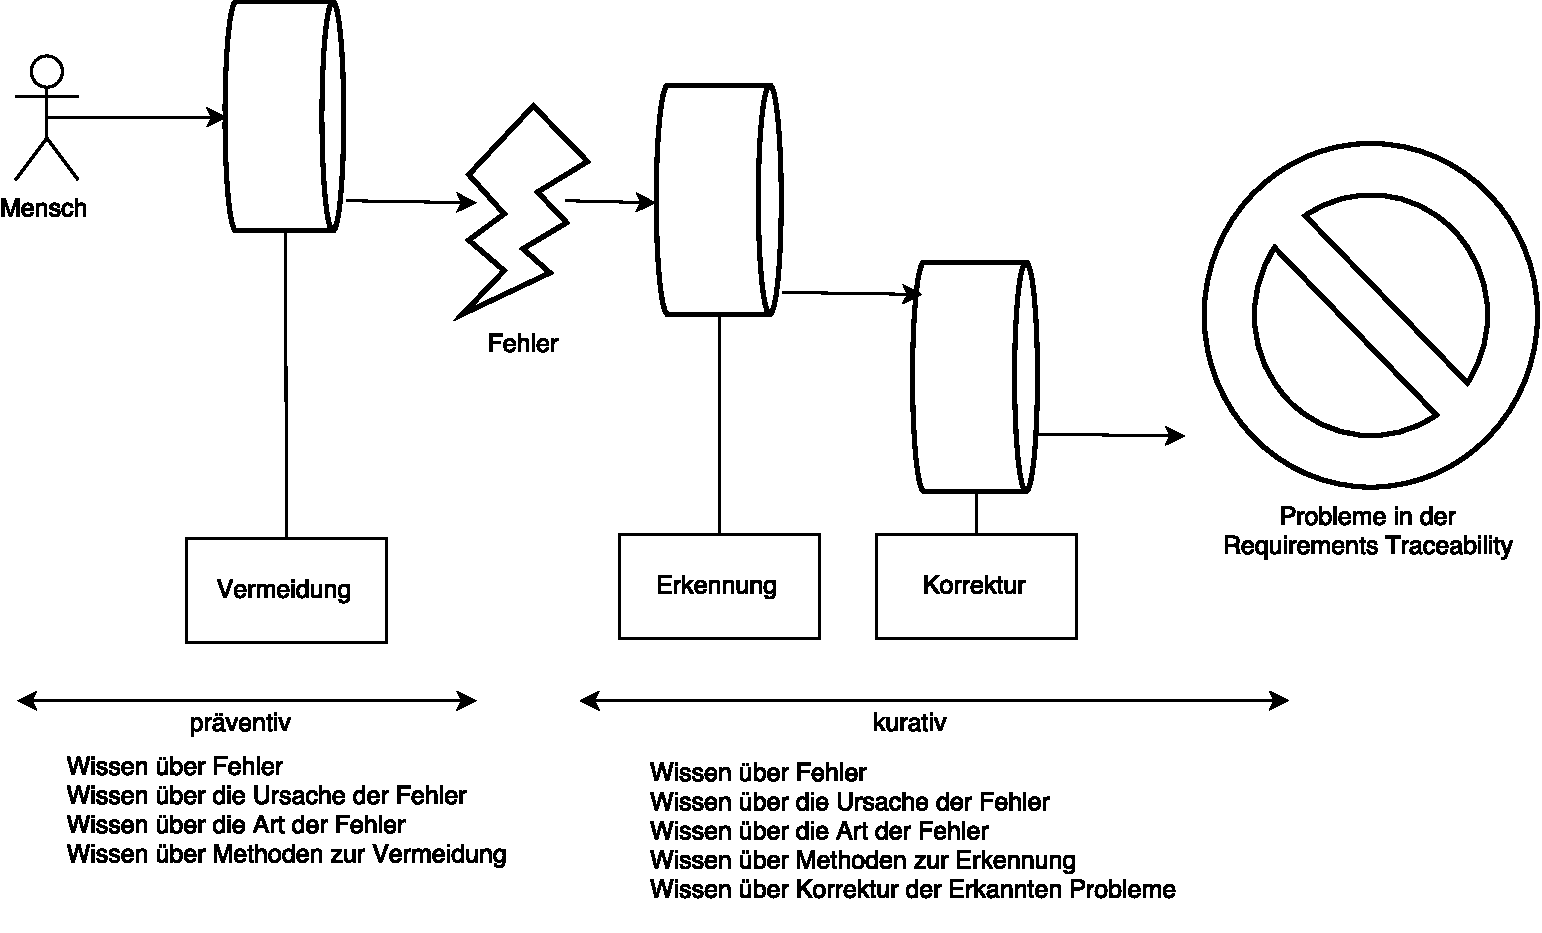
\includegraphics[width=3.4in]{Draft_Klassifikation_SLR.pdf}
  \caption{Draft Klassifikation für Forschungsfragen}
  \label{fig:abb3}
\end{figure}

DRAFT 14.06.2017

\begin{table*}
\centering
\begin{tabular}{cc}
\rowcolor[gray] {.6} \hline
Forschungsfrage & Motivation\\    \hline
... & Bestimmen der \\  \hline
... & Klassifikation bekannter Probleme in bekannter Literatur über Software Engineering \\ \hline
... & Finden von Methoden & Taxonomien die \\  \hline
\midrule


% Übergeordnetes Ziel
% Identifikation von Problemen in der Requirements Traceability die die Qualität mindern, um ihre Erkennung und Vermeidung zu verbessern.
% Muss noch eingesetzt werden. Vemutlich Einleitung? Planung?

% Fokus
Was für Arten von Problemen in der Requirements Traceability 

Gibt es  & B\\    \hline
2. Was für Typen von Problemen wurde in der bekannten Litera
Was für Arten von Problemen existieren in der Requirements Traceability?

    2.1 Gibt es Arten die die Qualität negativ beeinflussen können?
    2.2 
2. Welche Art von Problemen in der Requirements Traceability wurden identifiziert? & B\\    \hline
    1.1

\end{tabular}
\end{table*}




Methodologien
Enthält sie eine Art von Automatisierung
Was für eine Unterstützung
Wie trägt sie zur Verbesserung bei
Welche Fehler adressiert sie
Aufwand
Nutzen

Fokus : post-RS-traceability

Herausfinden:
- Was muss automatisiert werden
- Gibt es Modelle / Ansätze für die semi- / automatisierung?
- Welche Probleme sind noch ungelöst? Warum nicht / semi- / voll

Forschungsfragen:
- Welche Forschungsbereiche gibt es?
- Was für Probleme gibt es in den verschiedenen Bereichen der post-RS-traceability?
- Was für Ansätze / Modelle gibt es für die Pflege von post-RS-traceability?
- Welche davon sind automatisierbar? semi- und voll automatisierbar

\subsection{Ablauf (Review, Suchprozess)}

Review planen:

Forschungsfragen
Review Protokoll

Review ausführen:

Suchstrategie, Suchprozess, Methodik
Dokumentierung der Suche

Review Protokoll

Bestehende SLRs
Generellese Forschungsfeld
Zitationen von Gotel \& Finkelstein

\subsection{Kriterien (Inkusion-, Exklusion)}

Was sind die Kriterien für die Inkusion- / Exklusion- von Disserationen

\subsection{Analyse}

Wie wird analysiert, was sind die Methoden?
